\documentclass{article}
\usepackage{amsmath}
\usepackage{amssymb}
\usepackage{tikz}
\usetikzlibrary{fit}
\usetikzlibrary{calc}
\usetikzlibrary{shapes}
\usetikzlibrary{arrows}
\usetikzlibrary{positioning}
\usetikzlibrary{chains}
\usepackage{pgfplots}
\usepackage{pgfplotsthemetol}

\begin{document}

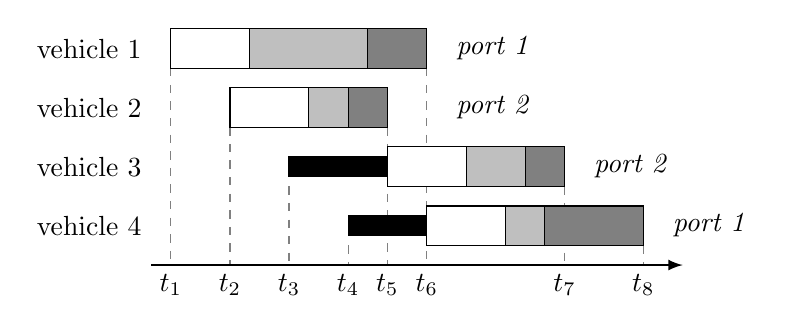
\begin{tikzpicture}
\tikzstyle{docking}  =[draw,fill=black!0!white];
\tikzstyle{unloading}=[draw,fill=black!25!white];
\tikzstyle{loading}  =[draw,fill=black!50!white];
\tikzstyle{waiting}  =[draw,fill=black];

\def\h{0.5}
\def\va{ 0.00}
\def\vb{-0.75}
\def\vc{-1.50}
\def\vd{-2.25}
\def\t{-2.50}

\node[below] at (0.00,\t) {$t_1$};
\draw[dashed,black!50!white] (0.00,\va) -- (0.00,\t);
\node[below] at (0.75,\t) {$t_2$};
\draw[dashed,black!50!white] (0.75,\vb) -- (0.75,\t);
\node[below] at (1.50,\t) {$t_3$};
\draw[dashed,black!50!white] (1.50,\vc) -- (1.50,\t);
\node[below] at (2.25,\t) {$t_4$};
\draw[dashed,black!50!white] (2.25,\vd) -- (2.25,\t);
\node[below] at (2.75,\t) {$t_5$};
\draw[dashed,black!50!white] (2.75,\vb) -- (2.75,\t);
\node[below] at (3.25,\t) {$t_6$};
\draw[dashed,black!50!white] (3.25,\va) -- (3.25,\t);
\node[below] at (5.00,\t) {$t_7$};
\draw[dashed,black!50!white] (5.00,\vc) -- (5.00,\t);
\node[below] at (6.00,\t) {$t_8$};
\draw[dashed,black!50!white] (6.00,\vd) -- (6.00,\t);

\draw[thick,->,-latex] (-0.25,\t) -- (6.50,\t);

\node[left] at (-0.25,\va+0.5*\h) {vehicle 1};
\node[left] at (-0.25,\vb+0.5*\h) {vehicle 2};
\node[left] at (-0.25,\vc+0.5*\h) {vehicle 3};
\node[left] at (-0.25,\vd+0.5*\h) {vehicle 4};

\draw[docking]   (0.00,\va) rectangle (1.00,\va+\h);
\draw[unloading] (1.00,\va) rectangle (2.50,\va+\h);
\draw[loading]   (2.50,\va) rectangle (3.25,\va+\h);

\draw[docking]   (0.75,\vb) rectangle (1.75,\vb+\h);
\draw[unloading] (1.75,\vb) rectangle (2.25,\vb+\h);
\draw[loading]   (2.25,\vb) rectangle (2.75,\vb+\h);

\draw[waiting]   (1.50,\vc + 0.25*\h) rectangle (2.75,\vc + 0.75*\h);
\draw[docking]   (2.75,\vc) rectangle (3.75,\vc+\h);
\draw[unloading] (3.75,\vc) rectangle (4.50,\vc+\h);
\draw[loading]   (4.50,\vc) rectangle (5.00,\vc+\h);

\draw[waiting]   (2.25,\vd + 0.25*\h) rectangle (3.25,\vd + 0.75*\h);
\draw[docking]   (3.25,\vd) rectangle (4.25,\vd+\h);
\draw[unloading] (4.25,\vd) rectangle (4.75,\vd+\h);
\draw[loading]   (4.75,\vd) rectangle (6.00,\vd+\h);

\node[right] at (3.50,\va+0.5*\h) {\textit{port~1}};
\node[right] at (3.50,\vb+0.5*\h) {\textit{port~2}};
\node[right] at (5.25,\vc+0.5*\h) {\textit{port~2}};
\node[right] at (6.25,\vd+0.5*\h) {\textit{port~1}};
\end{tikzpicture}

\end{document}